\chapter{Introdução} \label{chap:intro}

\section*{}

O objetivo desta dissertação é fornecer, de uma forma detalhada, toda a informação referente ao projeto, incluindo a revisão do estado da arte e também todos os conteúdos produzidos durante a realização do mesmo. Pretende-se que seja um documento o mais claro e simples possível para que seja necessário o mínimo de conhecimento específico para a sua compreensão. Todos os termos utilizados serão acompanhados de uma breve descrição para efeitos de contextualização.
Para melhor compreender o âmbito da dissertação, é apresentado neste capítulo o enquadramento e a motivação que levaram à escolha do tema e são também definidos os problemas que se pretendiam solucionar durante o projeto. Para além disso, é apresentada a estrutura da dissertação, permitindo assim criar desde já uma visão global do projeto.

\section{Contexto/Enquadramento} \label{sec:context}

Este projeto enquadra-se na área dos pagamentos móveis, com especial foco nos transportes públicos. Para além disso, está também enquadrada na área da bilhética, focando-se na compra e validação de títulos de viagem e assinaturas.
\\Por pagamento móvel entende-se o uso de um dispositivo móvel (telemóvel, PDA, \emph{tablet}) para iniciar, autorizar e confirmar uma troca de valor financeiro por bens ou serviços. \cite{Au2008141}
\\Um título de viagem corresponde ao objeto (físico ou virtual) que permite efetuar uma viagem dentro da rede de transportes para o qual foi concebido e o utilizador pode comprar um ou mais títulos de viagem de uma só vez, tendo em conta que apenas será utilizado um título por viagem.
\\Uma assinatura é uma modalidade que permite efetuar um número ilimitado de viagens dentro de uma determinada zona durante o período de tempo estipulado, habitualmente mensal.
\\A validação de títulos de viagem designa o processo que é realizado no início de cada viagem e realiza a ativação de um determinado título, confirmando a validade do mesmo e impedindo que seja usado novamente. Esta validação permite também verificar a adequação do mesmo título à viagem que se inicia. No caso das assinaturas, a validação verifica a adequação das mesmas à viagem e também se estão ainda ativas ou se o prazo definido já expirou.

~\\A adoção generalizada dos dispositivos móveis combinada com o aumento de funcionalidades está a mudar a forma como as pessoas utilizam os seus telemóveis. Começaram por ser essencialmente utilizados para realizar chamadas telefónicas e enviar mensagens de texto. No entanto, os telemóveis evoluíram para \emph{smartphones}, mudando totalmente a experiência móvel. Ver Figura~\ref{fig:evolution}. De facto, já é possível fazer pagamentos com telemóveis em vários países e nas mais variadas áreas, incluindo transportes públicos. O uso de telemóveis para pagamento oferece inúmeras vantagens, em comparação com o sistema tradicional, tais como a realização de operações em qualquer altura e lugar, a disponibilidade do serviço, o acesso remoto e ubíquo a serviços de pagamento e o evitar de filar. Para além disso, as funcionalidades dos telemóveis, como câmara, ecrã, som, GPS, etc. permitem a oferta de serviços adicionais que melhoram a experiência global do utilizador. Os dispositivos móveis podem ser usados para aplicar programas de fidelização, como cupões, prémios, publicidade inteligente, etc. \cite{Ferreira2013}
\\A indústria dos transportes enfrenta atualmente enormes desafios e ocupa um papel de destaque na política da União Europeia, visto este sector representar um papel importante na economia. Na União Europeia, emprega cerca de dez milhões de pessoas e representa à volta de 5\% do PIB. \cite{eurocomiss} Mobilidade é essencial para a economia, sociedade e para a qualidade de vida das pessoas. No entanto, esta mobilidade tem de ser sustentada e as novas tecnologias têm um papel importante neste fator. Para se melhorar a qualidade de vida nas cidades é importante fomentar o uso de transportes públicos, tirando proveito dos dispositivos móveis como simplificadores de todos os processos, tornando-os mais fáceis, cómodos e acessíveis, apresentando-se assim como um incentivo ao uso deste tipo de transportes. \cite{Ferreira2013}
\\Adicionalmente, o uso do telemóvel para pagar uma viagem pode melhorar a experiência global do passageiro. De facto, nos serviços de transportes públicos, as soluções de pagamento e bilhética sem contacto mostraram um aumento na satisfação do passageiro devido à sua facilidade e conveniência. \cite{NFCForum2011}
\\O uso de telemóveis nos transportes públicos irá revolucionar o sector, visto que estes permitem aos operadores oferecer aos seus clientes um leque de serviços através dum único canal. Utilizando o telemóvel, o utilizador pode aceder a informação em tempo-real, mapas, horários, partilhar opiniões e pagar as suas viagens. Por outro lado, os operadores beneficiam do facto de os serviços prestados serem fornecidos nos dispositivos dos utilizadores e não em infraestruturas próprias. Isto irá resultar em enormes ganhos operacionais e redução de custos. Mas também implica algumas alterações na cadeia de fornecimento, onde empresas de bilhética e fornecedores de equipamento são substituídos por bancos e operadoras móveis. \cite{Ferreira2013}

\begin{figure}[t]
  \begin{center}
    \leavevmode
    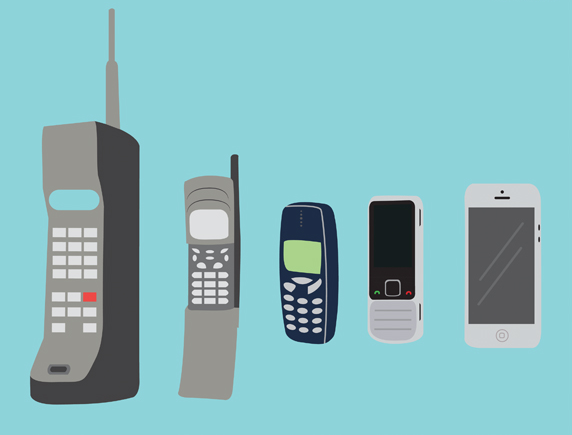
\includegraphics[scale=0.4]{evolution}
    \caption{Evolução do Telemóvel}
    \label{fig:evolution}
  \end{center}
\end{figure}

~\\É um trabalho realizado no âmbito de um projeto chamado MobiPag – Iniciativa Nacional para Pagamentos Móveis \cite{cedt}, financiado pelo QREN e que envolve várias empresas de tecnologia, universidades, bancos e operadoras moveis. A \Feup ficou responsável pelo desenvolvimento de um sistema de pagamentos móveis para os transportes públicos.
\\Durante o projeto, foi realizado um protótipo que envolve a STCP - Sociedade de Transportes Colectivos do Porto, SA, com o intuito de testar uma possível implementação de um sistema de pagamento e validação dos títulos de viagem utilizados pelos passageiros deste operador de transportes públicos. O protótipo foi desenvolvido em parceria com a OPT -  Optimização e Planeamento de Transportes, SA, empresa responsável pelo desenvolvimento dos produtos SMSBUS e MOVE-ME, entre outros relacionados com a gestão operacional do transporte coletivo urbano. \cite{OPT}
\\O protótipo desenvolvido é uma aplicação para dispositivos móveis com o sistema operativo Android, que permitirá aos passageiros efetuar a compra de títulos de viagem ou assinaturas e o respetivo pagamento, bem como validar os mesmos aquando da sua utilização nos transportes públicos. Para além disso permitirá visualizar o histórico de compras e validações efetuadas pelo passageiro e o saldo atual da carteira de títulos e da conta utilizada para os pagamentos.

\section{Motivação e Objetivos} \label{sec:goals}

Este projeto pretende facilitar os pagamentos e a validação de títulos de viagem nos transportes públicos na Área Metropolitana do Porto, tirando partido de dispositivos móveis. Por outro lado, pretende solucionar o problema causado pelo esquecimento, perda ou extravio de bilhetes, o que muitas vezes leva à necessidade da compra de um novo bilhete e títulos de viagem e, no caso da perda ou extravio, à impossibilidade de utilização dos títulos armazenados no bilhete perdido/extraviado.
\\A principal motivação deste trabalho é o elevado número de passageiros que utilizam os transportes públicos na Área Metropolitana do Porto. Durante o ano de 2012, cinquenta e quatro milhões e meio de passageiros utilizaram o Metro do Porto \cite{INE20130528} e quarenta e cinco milhões de passageiros viajaram nos autocarros da STCP (dados relativos a validações do sistema intermodal) durante o primeiro semestre de 2012. \cite{andante} Outros fatores de motivação são a criação de mobilidade sustentada, facilitar o dia-a-dia dos utilizadores de transportes públicos e, no limite, fomentar uma maior utilização destes transportes na Área Metropolitana do Porto.
\\Se o elevado número de passageiros serviu de base para a escolha da área de desenvolvimento, a escolha do meio tecnológico baseia-se no facto de que atualmente já uma em cada cinco pessoas acede à Internet no telemóvel \cite{INE20121106}, e também de cada vez mais ser menos provável deixar o telemóvel em casa. Um estudo efetuado revela que é mais provável as pessoas saírem de casa sem a carteira do que sem o telemóvel. \cite{NFCForum2011}.
\\Poder adicionar valor aos serviços já existentes é também uma grande motivação para o desenvolvimento deste projeto, apresentando-os como soluções únicas, atrativas, inovadoras e preferenciais.

~\\Os objetivos deste projeto são os seguintes:
\begin{itemize}
\item Criar uma nova forma de pagamento e validação de títulos de viagem, não substituindo os modelos atuais, servindo como um complemento dos mesmos;
\item Reduzir filas nas lojas Andante e postos de venda automáticos, descentralizando a operação de compra de títulos de viagem que muitas vezes causa longos períodos de espera, principalmente no início de cada mês, com a necessidade de renovação das assinaturas;
\item Reduzir custos de emissão e manuseamento de cartões, pois deixa de haver necessidade de um cartão físico, tudo está armazenado no dispositivo móvel do passageiro;
\item Conjugar informação relativa a cada viagem, apresentando detalhes ao passageiro, tal como a paragem até à qual pode viajar;
\item Fornecer informação estatística sobre os passageiros aos operadores de transportes, permitindo um melhor ajuste e planeamento de rotas e distribuição de veículos;
\item Possibilitar a realização de múltiplas operações em qualquer lugar e através do um único canal, concentrando um conjunto de serviços à distância de um clique, deixando de haver necessidade de consultar informações nos painéis informativos, comprar títulos de viagem num posto de venda automático ou num balcão e validar o título nas máquinas específicas para esse efeito;
\item Aumentar a satisfação geral dos utilizadores, trazendo-lhes mais comodidade e fornecendo-lhes um serviço que lhes permitirá poupar tempo e trabalho.
\end{itemize}

\section{Estrutura da Dissertação} \label{sec:struct}

Para além da introdução, esta dissertação contém mais 6 capítulos.
\\No Capítulo~\ref{chap:sota}, é descrito o estado da arte e são apresentados trabalhos realizados na área de pagamentos móveis, tanto a nível nacional como internacional. 
\\No Capítulo~\ref{chap:andante}, é descrito o sistema Andante, permitindo perceber e enquadrar a base do projeto.
\\No Capítulo~\ref{chap:projeto}, é descrito o projeto de uma forma mais detalhada, apresentando a sua estrutura e tecnologias a utilizar.
\\No Capítulo~\ref{chap:implement}, é apresentado o protótipo desenvolvido, especificando a sua implementação.
\\No Capítulo~\ref{chap:testes}, são especificados os testes realizados e os resultados obtidos.
\\No Capítulo~\ref{chap:concl} são apresentadas as conclusões obtidas durante a revisão do estado da arte, a implementação do projeto e os testes realizados.